\begin{problem}[Triangle Inequality and Cauchy-Schwarz]
Let $P(x,y,z)$ be a point on the unit sphere centered at the origin, so that $x^2 + y^2 + z^2 = 1$.

Prove:
\begin{enumerate}[label=(\roman*)]
    \item $|x| + |y| + |z| \geq 1$
    
    \item For any two vectors $\mathbf{a} = (a_1, a_2, a_3)$ and $\mathbf{b} = (b_1, b_2, b_3)$, the Cauchy-Schwarz inequality states:
    $$|\mathbf{a} \cdot \mathbf{b}| \leq |\mathbf{a}| \cdot |\mathbf{b}|$$
    
    Equivalently: $|a_1b_1 + a_2b_2 + a_3b_3| \leq \sqrt{a_1^2 + a_2^2 + a_3^2} \cdot \sqrt{b_1^2 + b_2^2 + b_3^2}$
    
    Derive this inequality from the dot product formula.
    
    \item $|x| + |y| + |z| \leq \sqrt{3}$
\end{enumerate}
\end{problem}

\begin{hint}
Use triangle inequality for part (i) and Cauchy-Schwarz with vector $(1,1,1)$ for part (iii).
\end{hint}

\begin{solution}[Sketch]
(i) By triangle inequality: $1 = |\mathbf{r}| \leq |x| + |y| + |z|$. (ii) From dot product: $|\mathbf{a} \cdot \mathbf{b}| \leq |\mathbf{a}||\mathbf{b}|$. (iii) Apply Cauchy-Schwarz with $\mathbf{a} = (|x|,|y|,|z|)$, $\mathbf{b} = (1,1,1)$: $|x| + |y| + |z| \leq \sqrt{x^2+y^2+z^2}\sqrt{3} = \sqrt{3}$.
\end{solution}

\vspace{1em}

\begin{problem}[Bimedians of Tetrahedron]
On the triangular pyramid (tetrahedron) $ABCD$, let:
\begin{itemize}
    \item $L$ is the midpoint of $AB$
    \item $M$ is the midpoint of $AC$
    \item $N$ is the midpoint of $AD$
    \item $P$ is the midpoint of $CD$
    \item $Q$ is the midpoint of $BD$
    \item $R$ is the midpoint of $BC$
\end{itemize}

\begin{center}
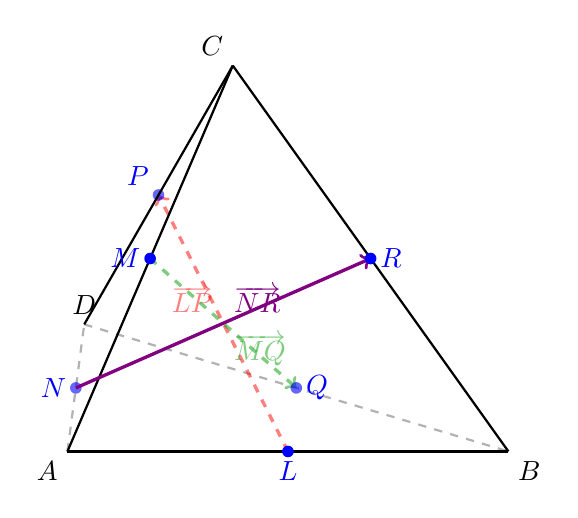
\begin{tikzpicture}[scale=1.4, line join=round]
    % Define vertices of tetrahedron (D repositioned higher and more forward)
    \coordinate (A) at (0,0,0);
    \coordinate (B) at (4,0,0);
    \coordinate (C) at (1.5,3.5,0);
    \coordinate (D) at (1.5,2.5,3.5);
    
    % Calculate midpoints
    \coordinate (L) at (2,0,0);        % midpoint of AB
    \coordinate (M) at (0.75,1.75,0);  % midpoint of AC
    \coordinate (N) at (0.75,1.25,1.75); % midpoint of AD
    \coordinate (P) at (1.5,3,1.75);   % midpoint of CD
    \coordinate (Q) at (2.75,1.25,1.75); % midpoint of BD
    \coordinate (R) at (2.75,1.75,0);  % midpoint of BC
    
    % Draw back/hidden edges (dashed)
    \draw[thick, dashed, gray!60] (A) -- (D);
    \draw[thick, dashed, gray!60] (D) -- (B);
    
    % Draw bimedian vectors (some behind)
    \draw[->, very thick, red, dashed, opacity=0.5] (L) -- (P) node[midway, above left, red] {$\overrightarrow{LP}$};
    \draw[->, very thick, green!60!black, dashed, opacity=0.5] (M) -- (Q) node[midway, below right, green!60!black] {$\overrightarrow{MQ}$};
    
    % Draw midpoints (back)
    \fill[blue, opacity=0.6] (N) circle (1.5pt);
    \fill[blue, opacity=0.6] (P) circle (1.5pt);
    \fill[blue, opacity=0.6] (Q) circle (1.5pt);
    
    % Draw front edges (solid)
    \draw[thick] (A) -- (B);
    \draw[thick] (A) -- (C);
    \draw[thick] (B) -- (C);
    \draw[thick] (C) -- (D);
    
    % Draw front bimedian vector
    \draw[->, very thick, violet] (N) -- (R) node[midway, above right, violet] {$\overrightarrow{NR}$};
    
    % Draw midpoints (front)
    \fill[blue] (L) circle (1.5pt);
    \fill[blue] (M) circle (1.5pt);
    \fill[blue] (R) circle (1.5pt);
    
    % Label vertices
    \node[below left] at (A) {$A$};
    \node[below right] at (B) {$B$};
    \node[above left] at (C) {$C$};
    \node[above] at (D) {$D$};
    
    % Label midpoints
    \node[below, blue] at (L) {$L$};
    \node[left, blue] at (M) {$M$};
    \node[left, blue] at (N) {$N$};
    \node[above left, blue] at (P) {$P$};
    \node[right, blue] at (Q) {$Q$};
    \node[right, blue] at (R) {$R$};
\end{tikzpicture}
\end{center}

\textit{Note: The three colored arrows show the bimedians $\overrightarrow{LP}$ (red), $\overrightarrow{MQ}$ (green), and $\overrightarrow{NR}$ (violet). Each bimedian connects the midpoint of one edge to the midpoint of the opposite edge.}

Let $\mathbf{b} = \overrightarrow{AB}$, $\mathbf{c} = \overrightarrow{AC}$ and $\mathbf{d} = \overrightarrow{AD}$.

\begin{enumerate}[label=(\roman*)]
    \item Show that $\overrightarrow{LP} = \frac{1}{2}(-\mathbf{b} + \mathbf{c} + \mathbf{d})$.
    
    \item It can be shown that:
    \[
    \overrightarrow{MQ} = \frac{1}{2}(\mathbf{b} - \mathbf{c} + \mathbf{d}) \quad \text{and} \quad \overrightarrow{NR} = \frac{1}{2}(\mathbf{b} + \mathbf{c} - \mathbf{d})
    \]
    (Do NOT prove these.)
    
    Prove that:
    \[
    |AB|^2 + |AC|^2 + |AD|^2 + |BC|^2 + |BD|^2 + |CD|^2 = 4\left( |LP|^2 + |MQ|^2 + |NR|^2 \right)
    \]
\end{enumerate}

\textit{Note: The segments $LP$, $MQ$, and $NR$ are called the bimedians of the tetrahedron. This problem proves that the sum of the squares of all six edges equals four times the sum of the squares of the three bimedians.}
\end{problem}

\begin{hint}
(i) Express $\overrightarrow{AL}$ and $\overrightarrow{AP}$ in terms of $\mathbf{b}$, $\mathbf{c}$, and $\mathbf{d}$, then find $\overrightarrow{LP} = \overrightarrow{AP} - \overrightarrow{AL}$.
(ii) Expand the left side as the sum of squared magnitudes of all six edges. Expand the right side by computing $4|LP|^2$, $4|MQ|^2$, and $4|NR|^2$ using dot products. Show both sides equal $3(b^2 + c^2 + d^2) - 2(\mathbf{b}\cdot\mathbf{c} + \mathbf{b}\cdot\mathbf{d} + \mathbf{c}\cdot\mathbf{d})$.
\end{hint}

\begin{solution}[Sketch]
(i) Since $L$ is midpoint of $AB$: $\overrightarrow{AL} = \frac{1}{2}\mathbf{b}$. Since $P$ is midpoint of $CD$: $\overrightarrow{AP} = \frac{1}{2}(\mathbf{c} + \mathbf{d})$. Therefore: $\overrightarrow{LP} = \overrightarrow{AP} - \overrightarrow{AL} = \frac{1}{2}(\mathbf{c} + \mathbf{d}) - \frac{1}{2}\mathbf{b} = \frac{1}{2}(-\mathbf{b} + \mathbf{c} + \mathbf{d})$.

(ii) LHS: The six edges are $AB$, $AC$, $AD$, $BC = \mathbf{c}-\mathbf{b}$, $BD = \mathbf{d}-\mathbf{b}$, $CD = \mathbf{d}-\mathbf{c}$.
\begin{align*}
LHS &= |\mathbf{b}|^2 + |\mathbf{c}|^2 + |\mathbf{d}|^2 + |\mathbf{c}-\mathbf{b}|^2 + |\mathbf{d}-\mathbf{b}|^2 + |\mathbf{d}-\mathbf{c}|^2 \\
&= 3(b^2 + c^2 + d^2) - 2(\mathbf{b}\cdot\mathbf{c} + \mathbf{b}\cdot\mathbf{d} + \mathbf{c}\cdot\mathbf{d})
\end{align*}

RHS: Using part (i) and the given expressions:
\begin{align*}
4|LP|^2 &= b^2 + c^2 + d^2 - 2\mathbf{b}\cdot\mathbf{c} - 2\mathbf{b}\cdot\mathbf{d} + 2\mathbf{c}\cdot\mathbf{d} \\
4|MQ|^2 &= b^2 + c^2 + d^2 - 2\mathbf{b}\cdot\mathbf{c} + 2\mathbf{b}\cdot\mathbf{d} - 2\mathbf{c}\cdot\mathbf{d} \\
4|NR|^2 &= b^2 + c^2 + d^2 + 2\mathbf{b}\cdot\mathbf{c} - 2\mathbf{b}\cdot\mathbf{d} - 2\mathbf{c}\cdot\mathbf{d}
\end{align*}

Summing: $RHS = 3(b^2 + c^2 + d^2) - 2(\mathbf{b}\cdot\mathbf{c} + \mathbf{b}\cdot\mathbf{d} + \mathbf{c}\cdot\mathbf{d}) = LHS$.
\end{solution}

\begin{takeaways}
\textbf{Key Concepts and Connections:}

\begin{itemize}
    \item \textbf{Bimedians of a Tetrahedron:} The three bimedians are segments connecting midpoints of opposite edges in a tetrahedron. This problem proves a beautiful relationship: the sum of squares of all six edge lengths equals four times the sum of squares of the three bimedian lengths.
    
    \item \textbf{Connection to Apollonius's Theorem:} This result is a 3D generalization of Apollonius's Theorem. In 2D, Apollonius's Theorem states that for a triangle with sides $a$, $b$, $c$ and median $m_c$ to side $c$:
    $$a^2 + b^2 = 2m_c^2 + \frac{c^2}{2}$$
    
    Equivalently: $2(a^2 + b^2 + c^2) = 4(m_a^2 + m_b^2 + m_c^2)$ where $m_a$, $m_b$, $m_c$ are the three medians.
    
    The tetrahedron bimedian theorem extends this median-edge relationship from triangles (2D) to tetrahedra (3D).
    
    \item \textbf{Algebraic Technique:} The solution demonstrates a powerful technique: expanding dot products systematically and observing how cross-terms cancel when summing. Notice how the coefficients $\pm 2$ in the dot product terms sum to $-2$ for each pair $(\mathbf{b}\cdot\mathbf{c})$, $(\mathbf{b}\cdot\mathbf{d})$, and $(\mathbf{c}\cdot\mathbf{d})$.
    
    \item \textbf{Symmetric Structure:} The three bimedian expressions have a beautiful symmetry:
    \begin{align*}
    \overrightarrow{LP} &= \frac{1}{2}(-\mathbf{b} + \mathbf{c} + \mathbf{d}) \\
    \overrightarrow{MQ} &= \frac{1}{2}(\mathbf{b} - \mathbf{c} + \mathbf{d}) \\
    \overrightarrow{NR} &= \frac{1}{2}(\mathbf{b} + \mathbf{c} - \mathbf{d})
    \end{align*}
    Each expression has exactly one negative sign, cycling through the three vectors. This symmetry guarantees that when we compute $|\overrightarrow{LP}|^2 + |\overrightarrow{MQ}|^2 + |\overrightarrow{NR}|^2$, the cross-terms will combine correctly.
    
    \item \textbf{Geometric Insight:} This theorem provides a metric relationship in tetrahedra, analogous to how Pythagoras relates sides in right triangles or how Apollonius relates medians in triangles. It's a fundamental identity in 3D geometry that can be used to prove other properties or solve optimization problems involving tetrahedra.
\end{itemize}
\end{takeaways}

\vspace{1em}

\begin{problem}[Triangle Intersection Ratios]
The diagram shows triangle $OQA$.

The point $P$ lies on $OA$ so that $OP : OA = 3 : 5$.

The point $B$ lies on $OQ$ so that $OB : OQ = 1 : 3$.

The point $R$ is the intersection of $AB$ and $PQ$.

The point $T$ is chosen on $AQ$ so that $O, R$ and $T$ are collinear.

Let $\mathbf{a} = \overrightarrow{OA}$, $\mathbf{b} = \overrightarrow{OB}$ and $\overrightarrow{PR} = k\overrightarrow{PQ}$ where $k$ is a real number.

\begin{enumerate}[label=(\roman*)]
    \item Show that $\overrightarrow{OR} = \frac{3}{5}(1-k)\mathbf{a} + 3k\mathbf{b}$.
    
    \item Writing $\overrightarrow{AR} = h\overrightarrow{AB}$, where $h$ is a real number, it can be shown that $\overrightarrow{OR} = (1-h)\mathbf{a} + h\mathbf{b}$. (Do NOT prove this.)
    
    Show that $k = \frac{1}{6}$.

    \item Find $\overrightarrow{OT}$ in terms of $\mathbf{a}$ and $\mathbf{b}$.
\end{enumerate}
\end{problem}

\begin{hint}
(i) Express $\overrightarrow{OR}$ as $\overrightarrow{OP} + \overrightarrow{PR}$. Use $\overrightarrow{OP} = \frac{3}{5}\mathbf{a}$ and $\overrightarrow{PQ} = -\overrightarrow{OP} + \overrightarrow{OQ}$ where $\overrightarrow{OQ} = 3\mathbf{b}$.
(ii) Equate coefficients of $\mathbf{a}$ and $\mathbf{b}$ from the two expressions for $\overrightarrow{OR}$. Use the relationship $3k = h$ and solve the system.
(iii) Since $O, R, T$ are collinear: $\overrightarrow{OT} = \lambda\overrightarrow{OR}$. Since $T$ is on $AQ$: $\overrightarrow{OT} = (1-\mu)\mathbf{a} + 3\mu\mathbf{b}$. Equate coefficients.
\end{hint}

\begin{solution}[Sketch]
(i) $\overrightarrow{OR} = \overrightarrow{OP} + k\overrightarrow{PQ}$. Since $\overrightarrow{OP} = \frac{3}{5}\mathbf{a}$ and $\overrightarrow{OQ} = 3\mathbf{b}$, we have:
$\overrightarrow{PQ} = -\frac{3}{5}\mathbf{a} + 3\mathbf{b}$.
Therefore: $\overrightarrow{OR} = \frac{3}{5}\mathbf{a} + k(-\frac{3}{5}\mathbf{a} + 3\mathbf{b}) = \frac{3}{5}(1-k)\mathbf{a} + 3k\mathbf{b}$.

(ii) Equating coefficients from both expressions:
For $\mathbf{b}$: $3k = h$.
For $\mathbf{a}$: $\frac{3}{5}(1-k) = 1-h$.
Substitute $h = 3k$ into second equation: $\frac{3}{5}(1-k) = 1-3k \Rightarrow 3(1-k) = 5(1-3k) \Rightarrow 3-3k = 5-15k \Rightarrow 12k = 2 \Rightarrow k = \frac{1}{6}$.

(iii) From part (ii): $\overrightarrow{OR} = \frac{3}{5}(1-\frac{1}{6})\mathbf{a} + 3(\frac{1}{6})\mathbf{b} = \frac{1}{2}\mathbf{a} + \frac{1}{2}\mathbf{b}$.

Since $O, R, T$ collinear: $\overrightarrow{OT} = \lambda\overrightarrow{OR} = \frac{\lambda}{2}(\mathbf{a} + \mathbf{b})$.

Since $T$ on $AQ$: $\overrightarrow{OT} = \mathbf{a} + \mu(\overrightarrow{OQ} - \mathbf{a}) = (1-\mu)\mathbf{a} + 3\mu\mathbf{b}$.

Equating coefficients: $\frac{\lambda}{2} = 1-\mu$ and $\frac{\lambda}{2} = 3\mu$.
From these: $1-\mu = 3\mu \Rightarrow \mu = \frac{1}{4}$.
Therefore: $\overrightarrow{OT} = (1-\frac{1}{4})\mathbf{a} + 3(\frac{1}{4})\mathbf{b} = \frac{3}{4}\mathbf{a} + \frac{3}{4}\mathbf{b} = \frac{3}{4}(\mathbf{a} + \mathbf{b})$.
\end{solution}

\vspace{1em}

\begin{problem}[Circle Intersection of Sets]
Let $A$ and $B$ be two distinct points in three-dimensional space. Let $M$ be the midpoint of $AB$.

Let $S_1$ be the set of all points $P$ such that $\overrightarrow{AP} \cdot \overrightarrow{BP} = 0$.

Let $S_2$ be the set of all points $N$ such that $\left| \overrightarrow{AN} \right| = \left| \overrightarrow{MN} \right|$.

The intersection of $S_1$ and $S_2$ is the circle $S$.

What is the radius of the circle $S$?

\begin{enumerate}[label=\Alph*.]
    \item $\displaystyle \frac{\left| \overrightarrow{AB} \right|}{2}$
    \item $\displaystyle \frac{\left| \overrightarrow{AB} \right|}{4}$
    \item $\displaystyle \frac{\sqrt{3} \left| \overrightarrow{AB} \right|}{2}$
    \item $\displaystyle \frac{\sqrt{3} \left| \overrightarrow{AB} \right|}{4}$
\end{enumerate}
\end{problem}

\begin{hint}
(Step 1) Recognize that $\overrightarrow{AP} \cdot \overrightarrow{BP} = 0$ defines a sphere with diameter $AB$ centered at $M$. (Step 2) The condition $|\overrightarrow{AN}| = |\overrightarrow{MN}|$ describes the perpendicular bisecting plane of segment $AM$. (Step 3) Use the Pythagorean relationship $r^2 + d^2 = R_{sphere}^2$ where $d$ is the distance from the sphere center to the plane.
\end{hint}

\begin{solution}[Sketch]
\textbf{Step 1: Analyze set $S_1$.} The condition $\overrightarrow{AP} \cdot \overrightarrow{BP} = 0$ means vectors $\overrightarrow{AP}$ and $\overrightarrow{BP}$ are perpendicular. The locus of points $P$ that subtend a right angle to segment $AB$ is a sphere with diameter $AB$. Center: $M$ (midpoint of $AB$). Radius: $R_{sphere} = \frac{1}{2}|\overrightarrow{AB}|$.

\textbf{Step 2: Analyze set $S_2$.} The condition $|\overrightarrow{AN}| = |\overrightarrow{MN}|$ describes points equidistant from $A$ and $M$, which is the perpendicular bisecting plane of segment $AM$.

\textbf{Step 3: Find intersection.} The intersection of a sphere (centered at $M$) and a plane is a circle. Using the Pythagorean relationship: $r^2 + d^2 = R_{sphere}^2$ where $d$ is the perpendicular distance from center $M$ to the plane.

\textbf{Step 4: Calculate distances.} Since the plane passes through the midpoint of $AM$, and $|\overrightarrow{AM}| = \frac{1}{2}|\overrightarrow{AB}|$, we have:
\[ d = \frac{1}{2}|\overrightarrow{AM}| = \frac{1}{2} \left( \frac{1}{2}|\overrightarrow{AB}| \right) = \frac{1}{4}|\overrightarrow{AB}| \]

\textbf{Step 5: Solve for radius $r$.}
\begin{align*}
    r^2 &= R_{sphere}^2 - d^2 = \left( \frac{|\overrightarrow{AB}|}{2} \right)^2 - \left( \frac{|\overrightarrow{AB}|}{4} \right)^2 \\
    &= \frac{|\overrightarrow{AB}|^2}{4} - \frac{|\overrightarrow{AB}|^2}{16} = \frac{4|\overrightarrow{AB}|^2 - |\overrightarrow{AB}|^2}{16} = \frac{3|\overrightarrow{AB}|^2}{16} \\
    r &= \frac{\sqrt{3}|\overrightarrow{AB}|}{4}
\end{align*}

Therefore, the answer is \textbf{D}.
\end{solution}

\vspace{1em}

\begin{problem}[Complex Numbers and Centroid]
The complex numbers $x$, $w$, and $z$ are all different and all have modulus 1 (i.e., they lie on the unit circle in the complex plane).

The \textbf{centroid} (also called the center of mass) of three points is the average of their positions, given by $G = \frac{1}{3}(x + w + z)$.

Prove that $\frac{1}{3}(x + w + z)$ is never a cube root of $xwz$.

\textit{Note: A cube root of $xwz$ is any complex number $K$ satisfying $K^3 = xwz$.}
\end{problem}

\begin{hint}
Show that the centroid has modulus strictly less than 1 (using the triangle inequality with strict inequality since the points are distinct), while any cube root of $xwz$ has modulus exactly 1.
\end{hint}

\begin{solution}[Sketch]
Given: $|x| = |w| = |z| = 1$ and $x, w, z$ are all different.

\textbf{Step 1: Find modulus of any cube root.} Let $K$ be any cube root of $xwz$, so $K^3 = xwz$. Taking modulus: $|K|^3 = |xwz| = |x||w||z| = 1 \cdot 1 \cdot 1 = 1$. Therefore $|K| = 1$. Thus, any cube root of $xwz$ lies on the unit circle.

\textbf{Step 2: Find modulus of centroid.} The centroid is $G = \frac{1}{3}(x + w + z)$. By triangle inequality: $|x + w + z| \leq |x| + |w| + |z| = 3$. Equality holds only if $x, w, z$ have the same argument (same direction), which means $x = w = z$. But they are given to be different, so strict inequality holds: $|x + w + z| < 3$. Therefore: $|G| = \left|\frac{x + w + z}{3}\right| < 1$.

\textbf{Conclusion:} Since $|G| < 1$ but $|K| = 1$ for any cube root $K$, we have $G \neq K$. Therefore, the centroid is never a cube root of the product.
\end{solution}

\vspace{1em}

\begin{problem}[Pyramid Centroid]
Consider a pyramid $SABCD$ with square base $ABCD$ and apex $S$. Let $H$ be the center of the square base (the intersection point of the diagonals $AC$ and $BD$).

\begin{center}
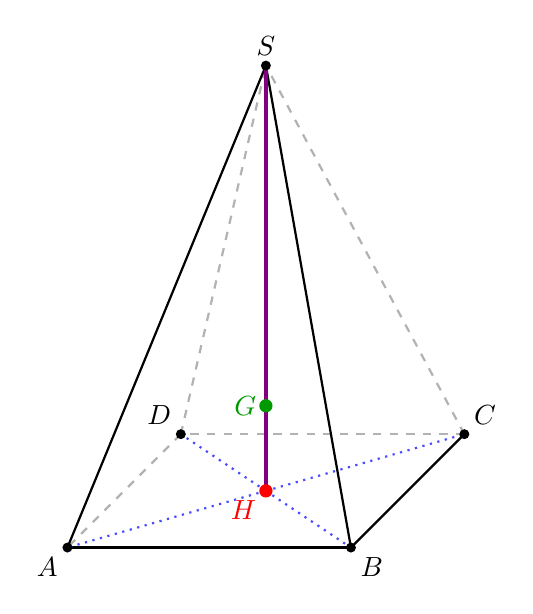
\begin{tikzpicture}[scale=1.2, line join=round, x={(1cm,0cm)}, y={(0.4cm,0.4cm)}, z={(0cm,1cm)}]
    % Define base vertices (square on xy-plane at z=0)
    \coordinate (A) at (0,0,0);
    \coordinate (B) at (3,0,0);
    \coordinate (C) at (3,3,0);
    \coordinate (D) at (0,3,0);
    
    % Define center of base
    \coordinate (H) at (1.5,1.5,0);
    
    % Define apex (directly above center)
    \coordinate (S) at (1.5,1.5,4.5);
    
    % Define centroid G (1/5 of the way from H to S)
    \coordinate (G) at (1.5,1.5,0.9);
    
    % Draw base square (all edges visible, some as dashed for depth)
    \draw[thick] (A) -- (B);
    \draw[thick] (B) -- (C);
    \draw[thick, dashed, gray!60] (C) -- (D);
    \draw[thick, dashed, gray!60] (D) -- (A);
    
    % Draw back edges to apex (dashed)
    \draw[thick, dashed, gray!60] (D) -- (S);
    \draw[thick, dashed, gray!60] (C) -- (S);
    
    % Draw base diagonals (dotted blue lines from H to vertices)
    \draw[dotted, blue!70, thick] (H) -- (A);
    \draw[dotted, blue!70, thick] (H) -- (B);
    \draw[dotted, blue!70, thick] (H) -- (C);
    \draw[dotted, blue!70, thick] (H) -- (D);
    
    % Draw line from H to S through G (dotted blue)
    \draw[dotted, blue!70, thick] (H) -- (S);
    
    % Draw front edges to apex (solid)
    \draw[thick] (A) -- (S);
    \draw[thick] (B) -- (S);
    
    % Highlight segment HG and GS in violet
    \draw[very thick, violet] (H) -- (G);
    \draw[very thick, violet] (G) -- (S);
    
    % Draw points
    \fill[black] (A) circle (1.5pt);
    \fill[black] (B) circle (1.5pt);
    \fill[black] (C) circle (1.5pt);
    \fill[black] (D) circle (1.5pt);
    \fill[black] (S) circle (1.5pt);
    \fill[red] (H) circle (2pt);
    \fill[green!60!black] (G) circle (2pt);
    
    % Label vertices
    \node[below left] at (A) {$A$};
    \node[below right] at (B) {$B$};
    \node[above right] at (C) {$C$};
    \node[above left] at (D) {$D$};
    \node[above] at (S) {$S$};
    \node[below left, red] at (H) {$H$};
    \node[left, green!60!black] at (G) {$G$};
\end{tikzpicture}
\end{center}

\textit{Note: $H$ (red) is the center of the square base, and $G$ (green) is the centroid of the pyramid. The blue dotted lines show vectors from $H$ to all five vertices.}

The centroid $G$ of the pyramid is the point such that:
$$\overrightarrow{GA} + \overrightarrow{GB} + \overrightarrow{GC} + \overrightarrow{GD} + \overrightarrow{GS} = \vec{0}$$

Show that $G$ lies on the line $HS$ with $\overrightarrow{HG} = \frac{1}{5}\overrightarrow{HS}$.
\end{problem}

\begin{hint}
Express each $\overrightarrow{GA_i}$ in terms of $\overrightarrow{GH}$ and $\overrightarrow{HA_i}$. Use the fact that $H$ is the center of the square base, so $\overrightarrow{HA} + \overrightarrow{HB} + \overrightarrow{HC} + \overrightarrow{HD} = \vec{0}$ by symmetry.
\end{hint}

\begin{solution}
\textbf{Finding the centroid $G$}

The centroid $G$ of the five vertices satisfies:
$$\overrightarrow{GA} + \overrightarrow{GB} + \overrightarrow{GC} + \overrightarrow{GD} + \overrightarrow{GS} = \vec{0}$$

Express each vector using the triangle rule: $\overrightarrow{GA} = \overrightarrow{GH} + \overrightarrow{HA}$:
\begin{align*}
\vec{0} &= \overrightarrow{GA} + \overrightarrow{GB} + \overrightarrow{GC} + \overrightarrow{GD} + \overrightarrow{GS} \\
&= (\overrightarrow{GH} + \overrightarrow{HA}) + (\overrightarrow{GH} + \overrightarrow{HB}) + (\overrightarrow{GH} + \overrightarrow{HC}) + (\overrightarrow{GH} + \overrightarrow{HD}) + (\overrightarrow{GH} + \overrightarrow{HS}) \\
&= 5\overrightarrow{GH} + (\overrightarrow{HA} + \overrightarrow{HB} + \overrightarrow{HC} + \overrightarrow{HD}) + \overrightarrow{HS}
\end{align*}

Since $H$ is the center of the square base, by symmetry the vectors from $H$ to the four base vertices cancel:
$$\overrightarrow{HA} + \overrightarrow{HB} + \overrightarrow{HC} + \overrightarrow{HD} = \vec{0}$$

(This follows because $H$ is the midpoint of both diagonals: $\overrightarrow{HA} = -\overrightarrow{HC}$ and $\overrightarrow{HB} = -\overrightarrow{HD}$.)

Therefore:
$$\vec{0} = 5\overrightarrow{GH} + \overrightarrow{HS}$$

Rearranging:
$$5\overrightarrow{GH} = -\overrightarrow{HS} = \overrightarrow{SH}$$

Therefore:
$$\overrightarrow{GH} = \frac{1}{5}\overrightarrow{SH}$$

Or equivalently:
$$\overrightarrow{HG} = \frac{1}{5}\overrightarrow{HS}$$

This shows that $G$ lies on the line segment $HS$, located $\frac{1}{5}$ of the way from $H$ to $S$.

\textbf{Answer:} The centroid $G$ divides the segment from the center of the base to the apex in the ratio $HG:GS = 1:4$.
\end{solution}

\vspace{1em}

\begin{problem}[Line-Sphere Intersection Points]
Find intersection points of line $\mathbf{r} = \mathbf{i} + 3\mathbf{j} - 4\mathbf{k} + t(\mathbf{i} + 2\mathbf{j} + 2\mathbf{k})$ and sphere $(x-1)^2 + (y-3)^2 + (z+4)^2 = 81$.
\end{problem}

\begin{hint}
Substitute parametric equations into sphere equation and solve resulting quadratic.
\end{hint}

\begin{solution}[Sketch]
Parametric: $x = 1+t$, $y = 3+2t$, $z = -4+2t$. Substitute: $(t)^2 + (2t)^2 + (2t)^2 = 81 \Rightarrow 9t^2 = 81 \Rightarrow t = \pm 3$. Points: $(4, 9, 2)$ when $t=3$ and $(-2, -3, -10)$ when $t=-3$.
\end{solution}

\vspace{1em}

\begin{problem}[Regular Octagon Vector Sum]
In regular octagon with side length 4, find magnitude of sum of vectors from midpoint of one side to all vertices.
\end{problem}

\begin{center}
\begin{tikzpicture}[scale=1.3, line join=round]
    % Calculate octagon vertices (radius chosen so side length = 4)
    % For regular octagon: side length s = 2R*sin(22.5°)
    % So R = s/(2*sin(22.5°)) ≈ 4/(2*0.3827) ≈ 5.226
    \def\R{5.226}
    
    % Define 8 vertices of regular octagon
    \foreach \i in {1,...,8} {
        \coordinate (P\i) at ({90 - (\i-1)*45}:\R);
    }
    
    % Define center O
    \coordinate (O) at (0,0);
    
    % Define midpoint A between P1 and P2
    \coordinate (A) at ($(P1)!0.5!(P2)$);
    
    % Draw octagon edges
    \foreach \i in {1,...,7} {
        \pgfmathtruncatemacro{\next}{mod(\i, 8) + 1}
        \draw[thick, blue!60] (P\i) -- (P\next);
    }
    \draw[thick, blue!60] (P8) -- (P1);
    
    % Draw vectors from A to all vertices (in red)
    \foreach \i in {1,...,8} {
        \draw[->, thick, red!70, opacity=0.6] (A) -- (P\i);
    }
    
    % Draw vector from A to O (highlighted)
    \draw[->, very thick, green!60!black] (A) -- (O) node[midway, right, green!60!black] {$\overrightarrow{AO}$};
    
    % Draw vectors from O to vertices (dashed, for reference)
    \foreach \i in {1,3,5,7} {
        \draw[->, dashed, gray!50, thin] (O) -- (P\i);
    }
    
    % Mark the side P1-P2 specially
    \draw[very thick, violet!80] (P1) -- (P2);
    
    % Draw points
    \fill[blue] (O) circle (2pt);
    \fill[red] (A) circle (2.5pt);
    \foreach \i in {1,...,8} {
        \fill[blue!80] (P\i) circle (1.8pt);
    }
    
    % Label vertices
    \node[above] at (P1) {$P_1$};
    \node[above right] at (P2) {$P_2$};
    \node[right] at (P3) {$P_3$};
    \node[below right] at (P4) {$P_4$};
    \node[below] at (P5) {$P_5$};
    \node[below left] at (P6) {$P_6$};
    \node[left] at (P7) {$P_7$};
    \node[above left] at (P8) {$P_8$};
    
    % Label center and midpoint
    \node[below, blue] at (O) {$O$};
    \node[above, red] at (A) {$A$};
\end{tikzpicture}
\end{center}

\textit{Note: The regular octagon has vertices $P_1, P_2, \ldots, P_8$, center $O$ (blue), and $A$ (red) is the midpoint of side $P_1P_2$ (shown in violet). Red arrows show vectors from $A$ to all eight vertices. The green arrow highlights $\overrightarrow{AO}$.}

\begin{hint}
Use symmetry: sum of vectors from center to vertices is zero. Express via center.
\end{hint}

\begin{solution}
\textbf{Step 1: Use vector decomposition via the center.}

For any point $A$ and the center $O$, we can write each vector from $A$ to a vertex $P_i$ as:
$$\overrightarrow{AP_i} = \overrightarrow{AO} + \overrightarrow{OP_i}$$

Summing over all 8 vertices:
\begin{align*}
\sum_{i=1}^{8} \overrightarrow{AP_i} &= \sum_{i=1}^{8} (\overrightarrow{AO} + \overrightarrow{OP_i}) \\
&= 8\overrightarrow{AO} + \sum_{i=1}^{8} \overrightarrow{OP_i}
\end{align*}

\textbf{Step 2: Apply symmetry to eliminate the sum from center.}

By symmetry of a regular octagon, the 8 vertices are evenly distributed around the center $O$. The vectors $\overrightarrow{OP_1}, \overrightarrow{OP_2}, \ldots, \overrightarrow{OP_8}$ point in directions separated by $45°$ and all have equal magnitude. Their vector sum is:
$$\sum_{i=1}^{8} \overrightarrow{OP_i} = \vec{0}$$

Therefore:
$$\sum_{i=1}^{8} \overrightarrow{AP_i} = 8\overrightarrow{AO}$$

\textbf{Step 3: Calculate the apothem $|AO|$.}

The apothem is the perpendicular distance from center to midpoint of a side. Consider the right triangle formed by $O$, midpoint $A$, and vertex $P_1$. The central angle between adjacent vertices is $45°$, so half this angle at $O$ is $22.5°$. With opposite side $|AP_1| = 2$ (half the side length) and adjacent side $|AO|$:
$$\tan(22.5°) = \frac{2}{|AO|} \quad \Rightarrow \quad |AO| = 2\cot(22.5°)$$

\textbf{Step 4: Evaluate $\cot(22.5°)$.}

Using the half-angle formula: $\tan(22.5°) = \sqrt{2} - 1$. Therefore:
$$\cot(22.5°) = \frac{1}{\sqrt{2} - 1} = \frac{\sqrt{2} + 1}{(\sqrt{2} - 1)(\sqrt{2} + 1)} = \sqrt{2} + 1$$

Thus: $|AO| = 2(\sqrt{2} + 1)$.

\textbf{Step 5: Find the final magnitude.}

From Step 2, we have $\sum_{i=1}^{8} \overrightarrow{AP_i} = 8\overrightarrow{AO}$.

Taking magnitudes:
$$\left|\sum_{i=1}^{8} \overrightarrow{AP_i}\right| = |8\overrightarrow{AO}| = 8|AO| = 8 \cdot 2(\sqrt{2} + 1) = 16(\sqrt{2} + 1)$$

\textbf{Answer:} The magnitude of the sum of vectors is $\boxed{16(\sqrt{2} + 1)}$ or approximately $\boxed{16(2.414) \approx 38.63}$.
\end{solution}



\vspace{1em}
